%%%%%%%%%%%%%%%%%%%%%%%%%%%%%%%%%%%%%%%%%
% Short Sectioned Assignment
% LaTeX Template
% Version 1.0 (5/5/12)
%
% This template has been downloaded from: http://www.LaTeXTemplates.com
% Original author: % Frits Wenneker (http://www.howtotex.com)
% License: CC BY-NC-SA 3.0 (http://creativecommons.org/licenses/by-nc-sa/3.0/)
% Modified by Alan G. Labouseur  - alan@labouseur.com, and Ryan Munger - ryan.munger1@marist.edu
%
%%%%%%%%%%%%%%%%%%%%%%%%%%%%%%%%%%%%%%%%%

%----------------------------------------------------------------------------------------
%	PACKAGES AND OTHER DOCUMENT CONFIGURATIONS
%----------------------------------------------------------------------------------------

\documentclass[letterpaper, 10pt]{article} 

\usepackage{tikz}
\usetikzlibrary{automata, positioning}
\usepackage[english]{babel} % English language/hyphenation
\usepackage{graphicx}
\usepackage[lined,linesnumbered,commentsnumbered]{algorithm2e}
\usepackage{listings}
\usepackage{float}
\usepackage{fancyhdr} % Custom headers and footers
\pagestyle{fancyplain} % Makes all pages in the document conform to the custom headers and footers
\usepackage{lastpage}
\usepackage{url}
\usepackage{xcolor}
\usepackage{titlesec}
\usepackage{ulem}

% Stolen from https://www.overleaf.com/learn/latex/Code_listing 
\definecolor{codegreen}{rgb}{0,0.6,0}
\definecolor{codegray}{rgb}{0.5,0.5,0.5}
\definecolor{codepurple}{rgb}{0.58,0,0.82}
\definecolor{backcolour}{rgb}{0.95,0.95,0.92}

\lstdefinestyle{mystyle}{
    backgroundcolor=\color{backcolour},   
    commentstyle=\color{codegreen},
    keywordstyle=\color{magenta},
    numberstyle=\tiny\color{codegray},
    stringstyle=\color{codepurple},
    basicstyle=\ttfamily\footnotesize,
    breakatwhitespace=false,         
    breaklines=true,                 
    captionpos=b,                    
    keepspaces=true,                 
    numbers=left,                    
    numbersep=5pt,                  
    showspaces=false,                
    showstringspaces=false,
    showtabs=false,                  
    tabsize=2
}
\lstset{style=mystyle, language=c++}


\fancyhead{} % No page header - if you want one, create it in the same way as the footers below
\fancyfoot[L]{} % Empty left footer
\fancyfoot[C]{page \thepage\ of \pageref{LastPage}} % Page numbering for center footer
\fancyfoot[R]{}

\renewcommand{\headrulewidth}{0pt} % Remove header underlines
\renewcommand{\footrulewidth}{0pt} % Remove footer underlines
\setlength{\headheight}{13.6pt} % Customize the height of the header

%----------------------------------------------------------------------------------------
%	TITLE SECTION
%----------------------------------------------------------------------------------------

\newcommand{\horrule}[1]{\rule{\linewidth}{#1}} % Create horizontal rule command with 1 argument of height

\title{	
   \normalfont \normalsize 
   \textsc{CMPT 432 - Spring 2025 - Dr. Labouseur} \\[10pt] % Header stuff.
   \horrule{0.5pt} \\[0.25cm] 	% Top horizontal rule
   \huge Lab 4 -- Analyzing Grammars \\     	    % Assignment title
   \horrule{0.5pt} \\[0.25cm] 	% Bottom horizontal rule
}

\author{Ryan Munger \\ \normalsize Ryan.Munger1@marist.edu}

\date{\normalsize\today} 	% Today's date.

\begin{document}

\maketitle % Print the title

%----------------------------------------------------------------------------------------
%   CONTENT SECTION
%----------------------------------------------------------------------------------------

% - -- -  - -- -  - -- -  -
\section{Crafting a Compiler}
\subsection{4.9	-- First and Follow set}
Compute First and Follow sets for the nonterminals of the following grammar.
\begin{figure} [h]
    \centering
    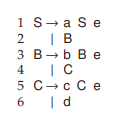
\includegraphics[width=0.3\linewidth]{4-9_grammar.png}
    \caption{Grammar for 4.9}
    \label{fig:enter-label}
\end{figure} \\
\textbf{First Set:} Set of all the possible terminals that can appear at the beginning of any string derived from a specific non-terminal. \\
\textbf{Follow Set:} Set of all the possible terminals that can immediately follow a specific non-terminal.
\begin{center}
\begin{table}[h]
\begin{tabular}{|c|c|c|c|}
\hline
\textbf{Production} & \textbf{Nullable} & \textbf{FIRST} & \textbf{FOLLOW} \\
\hline
    S & No & \{a, b, c, d\} & \{a, b, c, d, e\} \\
    B & No & \{b, c, d\} & \{b, c, d, e\} \\
    C & No & \{c, d\} & \{c, d, e\}\\
\hline
\end{tabular}
\end{table}
\end{center}

\subsection{5.10 -- Dangling Else Parse Trees}
Show the two distinct parse trees that can be constructed for: \\
\vspace{-.5cm}
\begin{center}
    \textit{if expr then if expr then other else other} \\
\end{center}
using the grammar below. For each parse tree, explain the correspondence of then and else.
\begin{figure} [h]
    \centering
    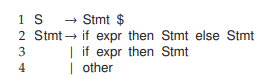
\includegraphics[width=0.6\linewidth]{5-10_Grammar.png}
    \caption{Grammar for 5.10}
    \label{fig:enter-label}
\end{figure} \\
\vspace{.3cm} \\
\begin{minipage}{0.48\textwidth} % Adjust width as needed
\textbf{Tree 1: }
\begin{verbatim}
S
-<Stmt>
--[if expr then]
--<Stmt>
---[if expr then]
---<Stmt>
----[Other]
--[else]
--<Stmt>
---[Other]
$
\end{verbatim}
\end{minipage}%
\hfill 
\begin{minipage}{0.5\textwidth}
\textbf{Tree 2: }
\begin{verbatim}
S
-<Stmt>
--[if expr then]
--<Stmt>
---[if expr then]
---<Stmt>
----[Other]
---[else]
---<Stmt>
----[Other]
$
\end{verbatim}
\end{minipage} \\
\vspace{.5cm} \\
Correspondence of \textit{then} \& \textit{else}: In tree \#1, the \textit{else} corresponds with the outer \textit{if expr then}. In tree \#2, the \textit{else} corresponds to the inner \textit{if expr then}. This is important as we need to know which \textit{if expr then} the \textit{else} is actually for.
\newpage

\section{Dragon Book}
\subsection{4.4.3 -- First and Follow set}
Compute FIRST and FOLLOW for the grammar below. \\

$S \to S S + | S S * | a$

\begin{center}
\begin{table}[h]
\begin{tabular}{|c|c|c|c|}
\hline
\textbf{Production} & \textbf{Nullable} & \textbf{FIRST} & \textbf{FOLLOW} \\
\hline
    S & No & \{a\} & \{+, *, a\} \\
\hline
\end{tabular}
\end{table}
\end{center}

\end{document}